\chapter{Visual scene context recognition through multimodal guidance}

In this chapter, we consider the task of recognizing visual scene context in media content by leveraging pre-trained multimodal information.  
\section{Role of scene as contextual signal}
Visual scene context refers to the global context in the image, including the relationship of the target objects with the environment/location and other co-occurring objects \cite{Bar2004VisualOI}, \cite{Qiao2021ObjectLevelSC}. Visual scene context drives the likelihood of finding particular objects spatially co-located with each other. For example, as shown in Fig \ref{station_kitchen}, utensils are more likely to be present in the kitchen as compared to the train station. 
Apart from the domain of natural scenes, understanding the visual scene context is also important in the case of media content \cite{CMI} esp. movies and curated short content like advertisements. 
\par
In cinematic terms, \textit{mis-en-scene} \cite{Bordwell1979FilmAA} refers to how the different elements of a film are depicted and arranged in front of camera. Key components of \textit{mis-en-scene} include the actors with their different styles, \textbf{visual scenes} where the interactions take place, set design including lighting and camera placement, and the accompanying costumes and makeup of the artists. The visual scene is considered a crucial component since it sets the mood and provides a background for the various actions performed by the actors in the scene. Visual scenes in movies are often tied to social settings like weddings, birthday parties, and workplace gatherings that provide information about character interactions. Accurate recognition of visual scenes can help in uncovering the bias involved in the portrayal of under-represented characters vis-a-vis different scenes, e.g., fewer women shown in the office as compared to the kitchen. For content tagging tasks like genre classification, visual scenes provide context information like battlefield portrayals in action/adventure movies, space-shuttle in sci-fi movies, or courtrooms in dramas.
\par 
In the following section, we highlight certain challenges associated with visual scene recognition, especially w.r.t. movies.
\begin{figure}[h!]
    \centering 
     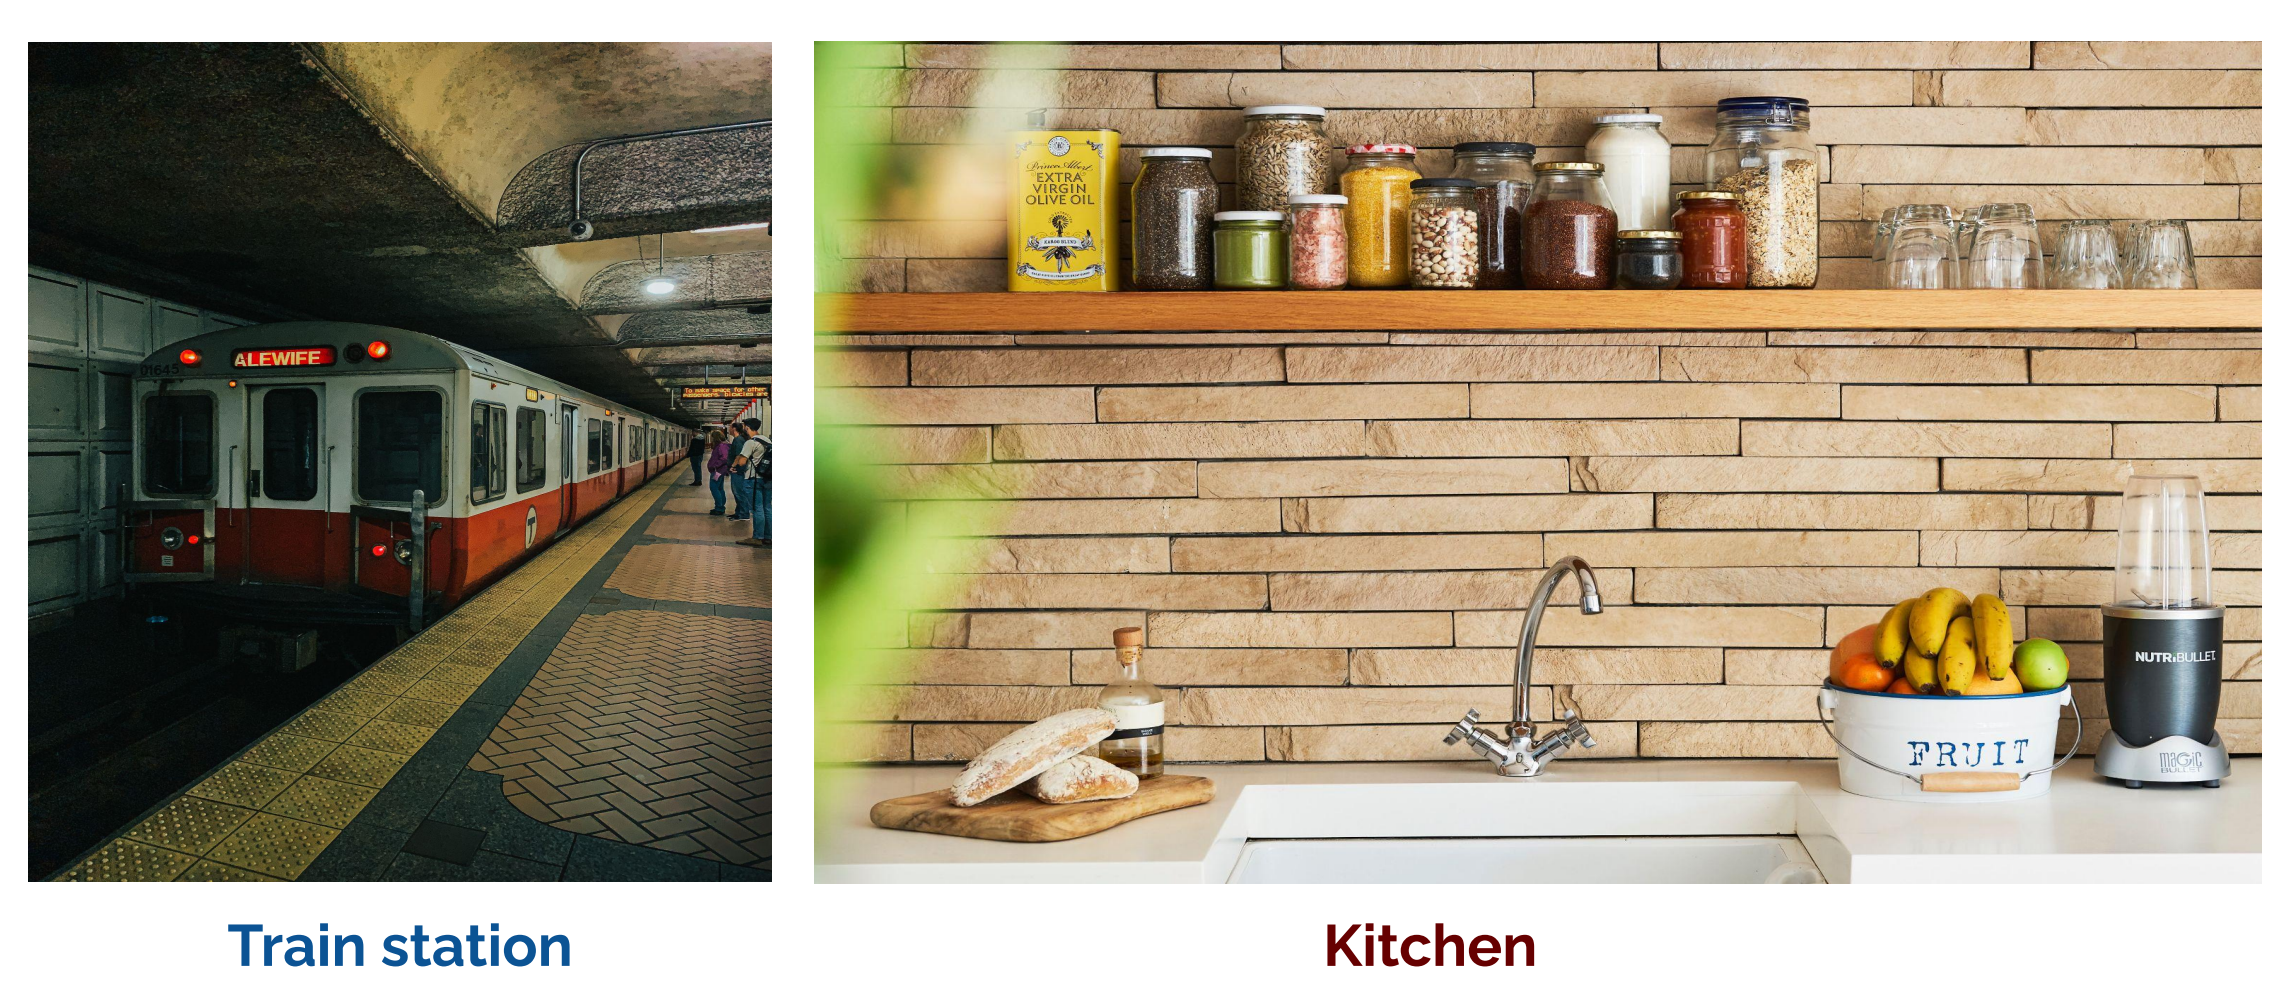
\includegraphics[width=0.6\linewidth]{figures/train_station_kitchen.png}
     \caption{Difference between visual scenes - train station and kitchen in terms of object placements.}
     \label{station_kitchen}
\end{figure}
% Use reference: \textit{Structure Inference Net: Object Detection Using Scene-Level Context and Instance-Level Relationships} here.
\section{Movies vs Natural scenes}
Visual scene recognition, in the case of static images, is primarily driven by natural scenes due to large-scale datasets like SUN397 \cite{Xiao2010SUNDL} and Places-2\cite{zhou2017places}. However, there are certain inherent challenges in visual scene recognition for movies that need to be addressed, as shown in Fig \ref{Intro figure}.
\begin{figure}[!h]
 \centering
  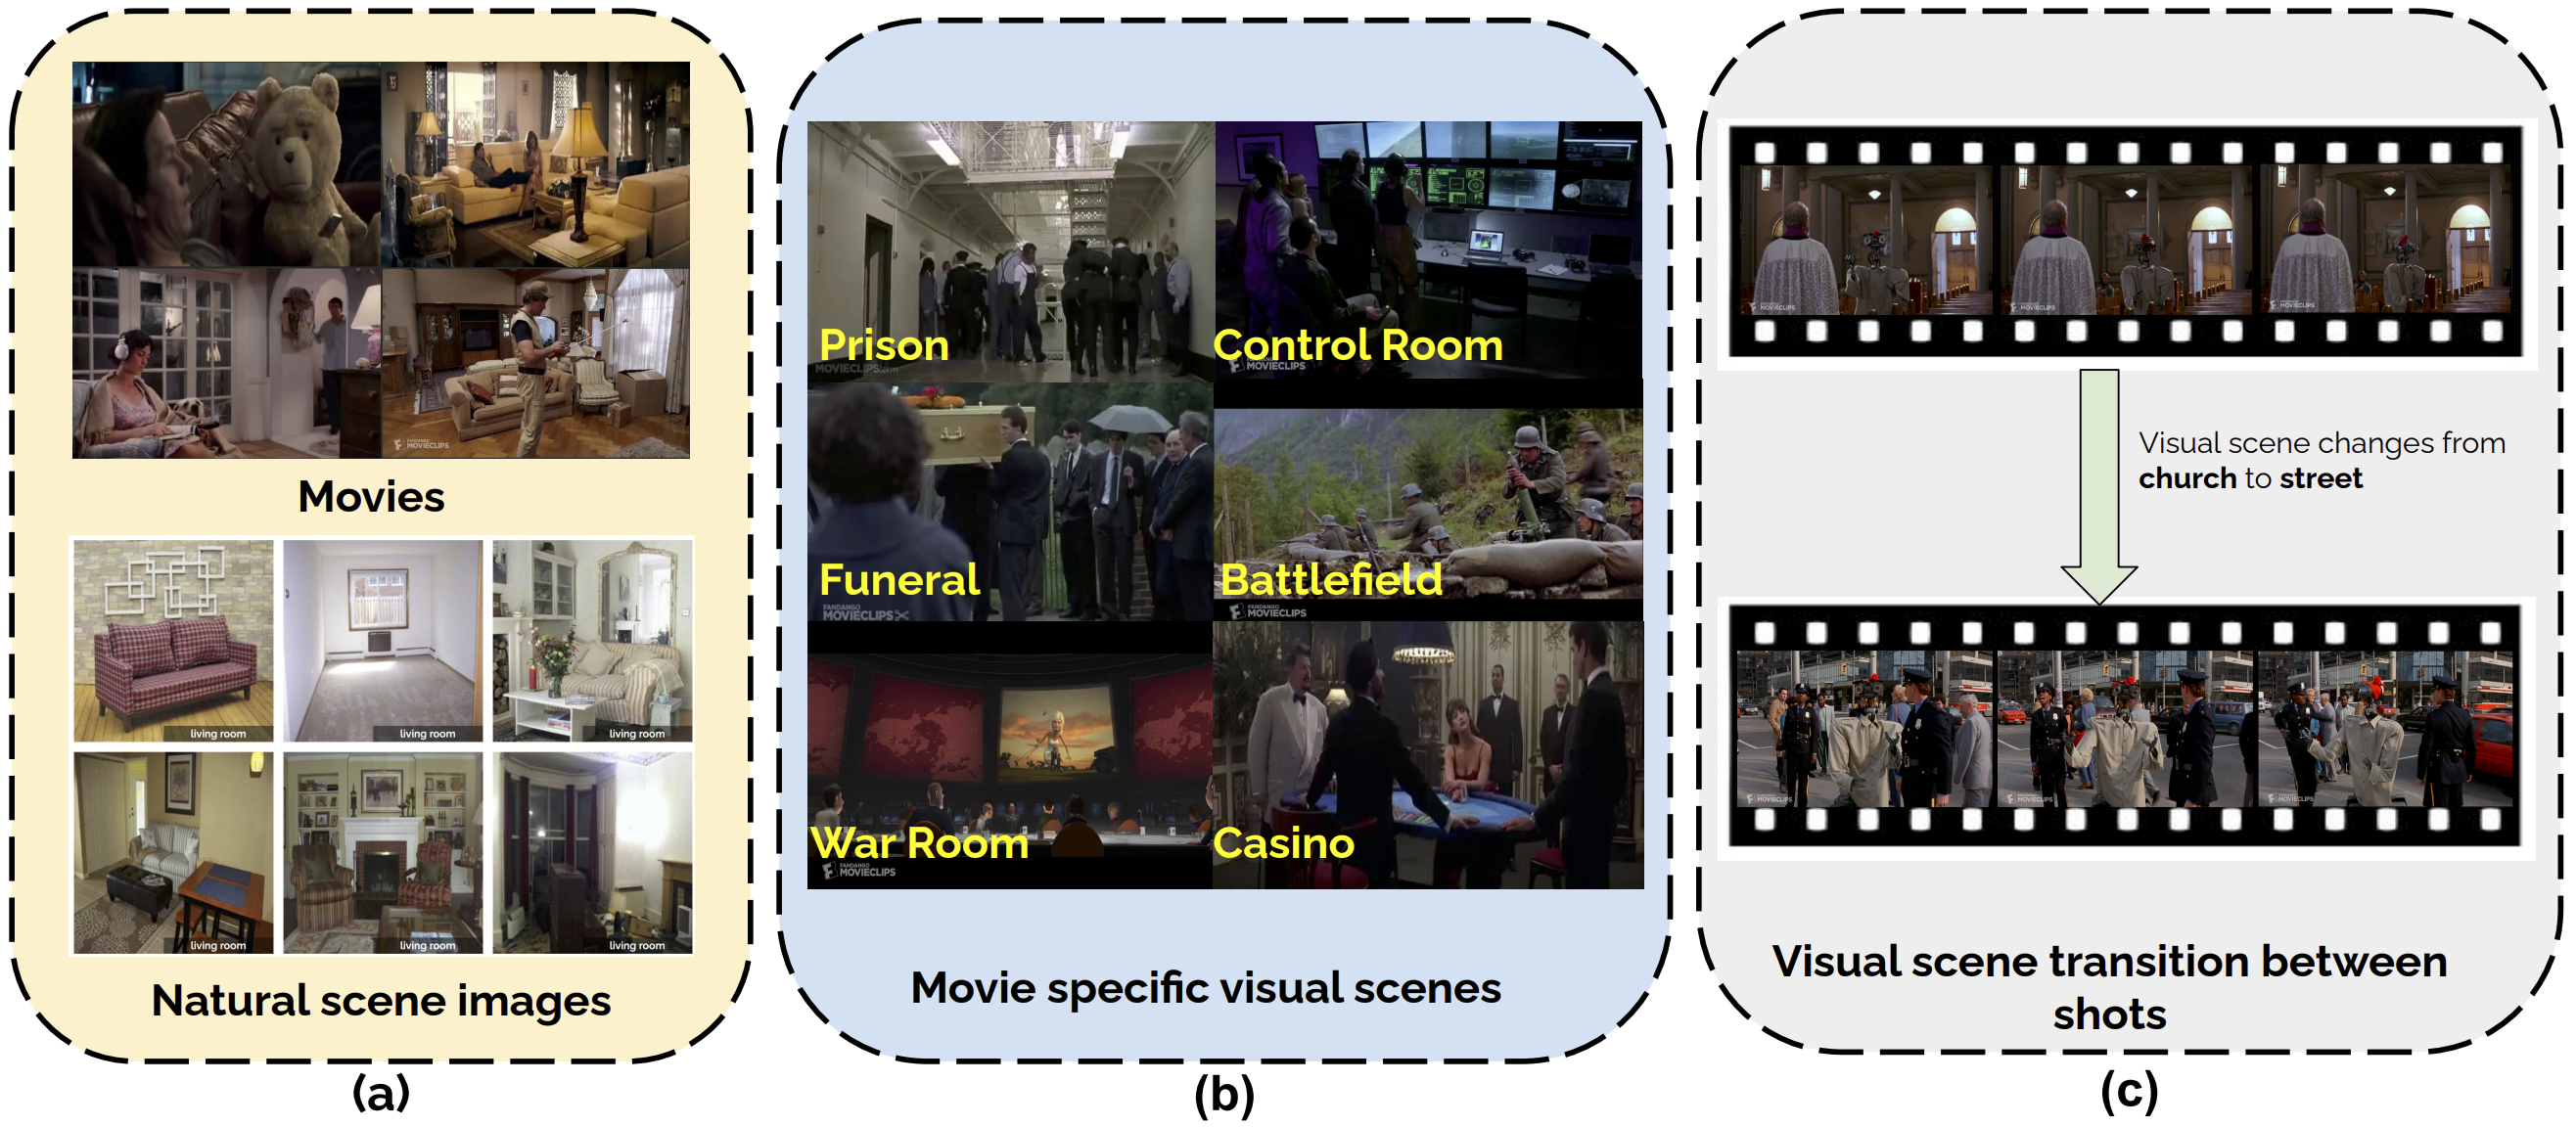
\includegraphics[width=0.8\linewidth]{figures/Introduction_Figure.png}
  \caption{Overview diagram highlighting the challenges associated with visual scene recognition in movies (a) Domain mismatch between Natural scene images,(Source: \url{http://places2.csail.mit.edu/explore.html}) vs frames from Movies for \textbf{living room} (b) Movie centric visual scene classes like prison, control room etc that are absent from existing taxonomies (c) Change in visual scene between shots in the same movie clip.}
  \label{Intro figure}
\end{figure}
\textbf{\underline{Domain mismatch - scene images vs. movie frames:}} Visual scenes depicted in movies are distinct compared to natural scenes due to increased focus on actors, multiple activities, and viewpoint variations like extreme closeup, wide-angle shots etc. An example is shown in Fig.~\ref{Intro figure} (a) for images from Places2 dataset \cite{zhou2017places} and movie frames from Condensed Movies dataset \cite{bain2020condensed}.\\
\textbf{\underline{Lack of completeness in scene taxonomy:}} Movies depict both real-life and fictional scenarios that span a wide variety of visual scenes. As shown in Fig.~\ref{Intro figure}(b), certain movie-centric visual scene classes like \textit{battlefield}, \textit{control room}, \textit{prison}, \textit{war room}, \textit{funeral}, \textit{casino} are absent from existing public scene taxonomies associated with natural scene image and video datasets.\\
\textbf{\underline{Lack of shot-specific visual scene annotations:}} Existing datasets like Condensed Movies \cite{bain2020condensed} and VidSitu \cite{Sadhu_2021_CVPR} provide a {\em single} visual scene label for the entire movie clip (around 2 minutes long), obtained through descriptions provided as part of YouTube channel Fandango Movie clips \footnote{https://www.youtube.com/channel/UC3gNmTGu-TTbFPpfSs5kNkg}. In Fig.~\ref{Intro figure} (c), the provided description: \textit{Johnny Five (Tim Blaney) searches for his humanity in the \textbf{streets} of New York.} mentions only the visual scene \textbf{street}, while the initial set of events takes place inside \textbf{church}. Instead of considering a single scene label for the entire movie clip, shot-level visual scene annotation can help in tracking the scene change from \textbf{church} to \textbf{street}.
\section{Contributions}
In our work, we consider shots within a given movie clip as the fundamental units for visual scene analysis since shots consist of consecutive set of frames related to the same content, whose starting and ending points are triggered by recording using a single camera \cite{SBD}. Our contributions are as follows:
Our contributions are as follows:
\begin{itemize}
\item \textbf{Language guided Movie-centric scene taxonomy:} We develop a movie-centric scene taxonomy by leveraging scene headers (sluglines) from movie scripts (language-based sources) and existing video datasets with scene labels like HVU\cite{diba_large_2020}. 
\item \textbf{Automatic shot tagging:} We utilize our generated scene taxonomy to automatically tag around 1.12M shots from 32K movie clips using a pretrained vision-language model called CLIP \cite{CLIP} based on a frame-wise aggregation scheme.  
\item \textbf{Multi-label scene classification:} We develop multi-label scene classification baselines using the shot-level tagged dataset called MovieCLIP and evaluate them on an independent shot-level dataset curated by human experts. 
\item \textbf{Downstream tasks:} We further extract feature representations from the baseline models pretrained on MovieCLIP and explore their applicability in diverse downstream tasks of multi-label scene and movie genre classification from web videos \cite{diba_large_2020} and trailers \cite{2019Moviescope}, respectively. 
\end{itemize}
\section{Related work}
\textbf{Image datasets for visual scene recognition:}
Image datasets for scene classification like MIT Indoor67 \cite{IndoorScenes} relied on categorizing a finite set of (67) indoor scene classes. A broad categorization into indoor, outdoor (natural) and outdoor (man-made) groups for 130K images across 397 subcategories was introduced by the SUN dataset \cite{xiao_sun_2016}. For large-scale scene recognition, the Places dataset \cite{zhou2017places} was developed with 434 scene labels spanning 10 million images. The scene taxonomy considered in the Places dataset was derived from the SUN dataset, followed by the careful merging of similar pairs. It should be noted that the curation of large-scale visual scene datasets like Places relied on crowd-sourced manual annotations over multiple rounds.\\
\section{Role of multi-modality:}
    \subsection{Language driven taxonomy curation}
    \subsection{Usage of vision-language models}
    \subsubsection{CLIP: Learning Transferable Visual Models From Natural Language Supervision}
    \subsection{MovieCLIP dataset}
    \subsubsection{CLIP-based visual tagging}
    \subsubsection{Analysis of CLIP tagging}
    \subsubsection{Quality estimation through human verification}
\section{Experiments and Results:}
\subsection{Experimental Setup}
\subsection{Visual scene recognition - Movies}
\subsection{Downstream tasks}
\subsubsection{Visual scene recognition - web videos}
\subsubsection{Multi label genre classification - movie trailers}
\subsubsection{Impact of MovieCLIP pretraining}
\section{Ethical implications}
\section{Conclusion}
